% !TEX TS-program = LuaLaTeX

\documentclass[10pt]{beamer}
\usepackage{booktabs,refstyle,siunitx,multicol,tikz}
\usepackage[style=numeric-comp,sorting=none,maxnames=99]{biblatex}
\renewcommand*{\bibfont}{\fontsize{5}{5}\selectfont}
\setlength{\biblabelsep}{0.1em}

\setbeamertemplate{navigation symbols}{}

\definecolor{maincolour}{HTML}{F57D1D}
\definecolor{darkcolour}{HTML}{BE1E2D}
\definecolor{lightcolour}{HTML}{FDBD0A}

\setbeamercolor{alerted text}{fg=lightcolour}
\setbeamercolor{structure}{fg=maincolour}
\setbeamercolor{palette primary}{bg=maincolour, fg=white}
\setbeamercolor{palette secondary}{bg=maincolour!80, fg=white}
\setbeamercolor{palette tertiary}{bg=maincolour!60, fg=white}
\setbeamercolor{title}{fg=maincolour}
\setbeamercolor{frametitle}{fg=maincolour}

\usepackage{fontspec}
\setsansfont{palatino-sans}

\IfFileExists{wspr.tex}{
  % WR live/local copies
  \bibliography{acoustics,wspr-conf}
}{
  % extracted with `make bib`
  \bibliography{in26-references}
}

\begin{document}

\title{%
\vspace*{-0.5cm}\par
\includegraphics[height=2cm]{fig/conf-logo.pdf}\par
Introducing aubellhop: a modern Python interface to the Bellhop underwater acoustics ray tracing tool}
\author{    William S.P. Robertson,\textsuperscript{1}
    Mandar Chitre,\textsuperscript{2}\\
    Chung T.C. Fang,\textsuperscript{1}
    Anthony C. Zander\textsuperscript{1}
}
\date{August 12, 2026}
\begin{frame}

\maketitle

\medskip

  \begin{flushleft}

\tiny
    \begin{multicols}{3} % <= choose the number of columns
    \makebox[0pt][r]{\textsuperscript 1}{%
      Acoustics, Vibrations, and Control Group,\\
      School of Elec.\ and Mech.\ Engineering\\
      Adelaide University\\ SA, Australia\\
    }
    \makebox[0pt][r]{\textsuperscript 2}{%
      Acoustic Research Laboratory,\\
      Tropical Marine Science Institute\\
      National University of Singapore\\
      Singapore
    }
    \includegraphics[height=1cm]{fig/uni-logo.pdf}
    \end{multicols}
  \end{flushleft}

\end{frame}


\begin{frame}
\frametitle{Overview}

\begin{columns}
\column{0.4\textwidth}
\parskip3ex\relax
\tableofcontents
\column{0.6\textwidth}
\centerline{\includegraphics[width=1.1\linewidth]{fig/bellhop-structure.pdf}}
\end{columns}
\end{frame}

\section{Outline of Bellhop}

\begin{frame}
\sectionpage
\end{frame}

\begin{frame}
\frametitle{Bellhop is a ray/beam tracing program}
\begin{itemize}
\item Originally released in the 1980s by Michael Porter et al. \parencite{porter2025-foa}
\item Continues to be used and extended as a research tool \parencite{oliveira2021-fms}
\end{itemize}
\begin{figure}
\centering
\includegraphics[width=0.45\linewidth]{fig/erays-2d}\hfil
\includegraphics[width=0.49\linewidth]{fig/erays-3d}
\caption{Underwater eigenrays between a source and receiver, calculated using constant speed of sound (left); equivalent 2.5D analysis calculated in Bellhop3D (right).}
\figlabel{erays}
\end{figure}
\end{frame}

\begin{frame}
\frametitle{Bellhop does rays\dots}
\centering
\includegraphics[height=0.8\textheight]{fig/demo-rays.pdf}
\end{frame}
\begin{frame}
\frametitle{Bellhop does eigenrays\dots}
\centering
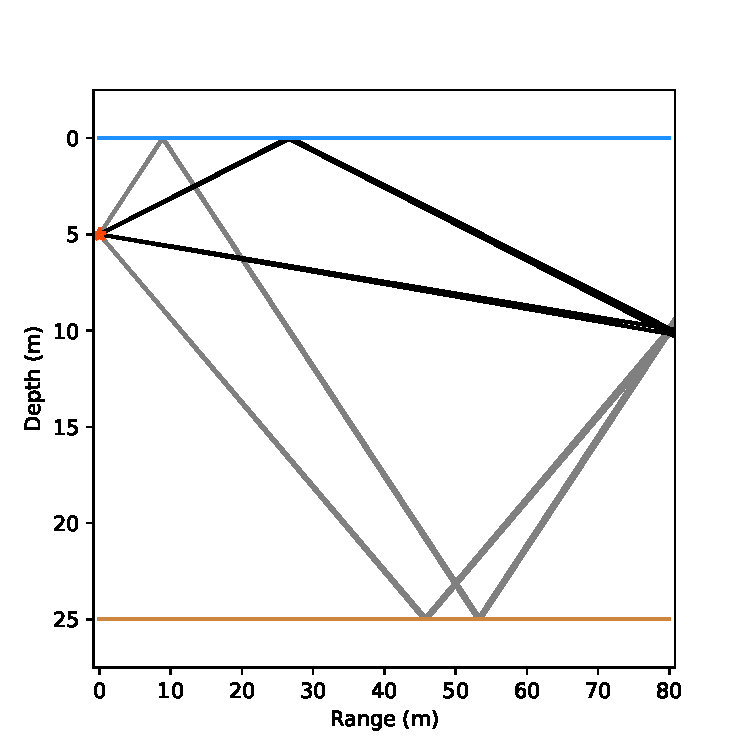
\includegraphics[height=0.8\textheight]{fig/demo-erays.pdf}
\end{frame}
\begin{frame}
\frametitle{\dots from which we get arrivals\dots}
\centering
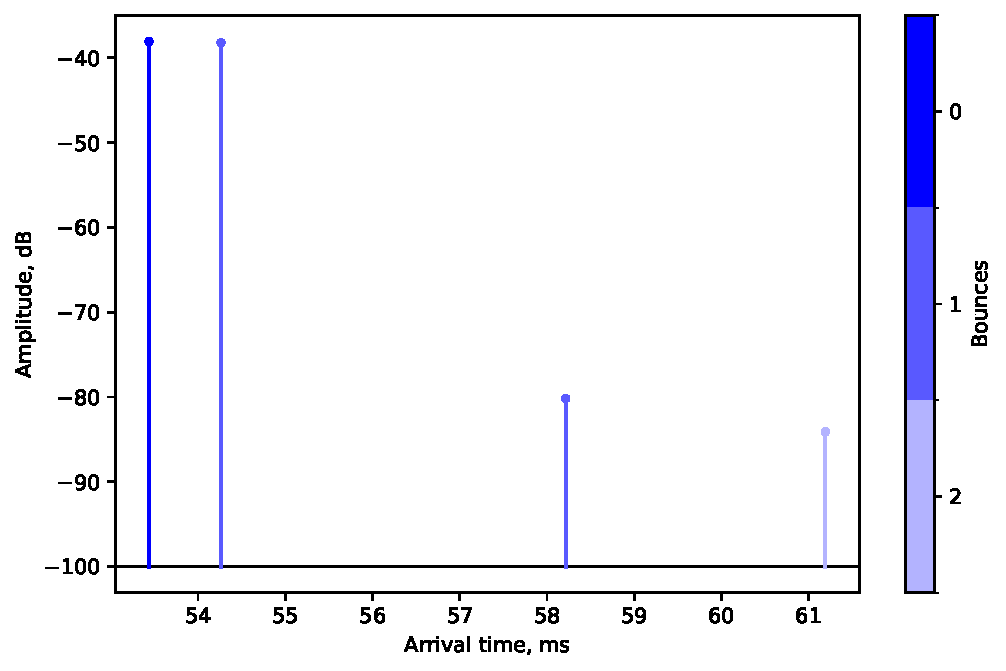
\includegraphics[height=0.8\textheight]{fig/demo-arr.pdf}
\end{frame}
\begin{frame}
\frametitle{Bellhop does transmission loss\dots}
\centering
\includegraphics[height=0.8\textheight]{fig/demo-tlc.pdf}
\end{frame}
\begin{frame}
\frametitle{\dots incoherent\dots}
\centering
\includegraphics[height=0.8\textheight]{fig/demo-tli.pdf}
\end{frame}
\begin{frame}
\frametitle{\dots semi-coherent\dots}
\centering
\includegraphics[height=0.8\textheight]{fig/demo-tls.pdf}
\end{frame}
\begin{frame}
\frametitle{\dots and different beam/ray types (gaussian-cartesion)\dots}
\centering
\includegraphics[height=0.8\textheight]{fig/demo-tls-gc.pdf}
\end{frame}

\begin{frame}
\frametitle{Ray/beam tracing implementations}

The main Bellhop developments:
\begin{itemize}
\item \alert{bellhop} and \alert{bellhop3d}, in \texttt{Acoustics Toolbox} by \textcite{porter2024-at}\\ (Heat, Light, and Sound Research, Inc.)
\item \alert{{bellhopcpp}} and \alert{{bellhopcuda}} by \textcite{jaffe2025-bellhopcuda}\\ (Marine Physical Lab at Scripps Oceanography)
\end{itemize}
Competitors or other ray/beam tracers, e.g.:
\begin{itemize}
\item \alert{{TRACEO3D}} by \textcite{calazan2017-traceo3d}\\ (LARSyS, University of Algarve, Portugal)
\item \alert{dBSea} by Marshall Day Acoustics and Irwin Carr Consulting (\url{https://www.dbsea.co.uk})
\end{itemize}
\& other proprietary software\dots
\end{frame}

\begin{frame}
\frametitle{Interfaces to Bellhop}
\begin{itemize}
\item The raw Fortran interfaces
\item \texttt{Acoustics Toolbox} (Matlab) by \textcite{porter2024-at}
\item \texttt{Actup} (Matlab) by \textcite{duncan2025-actup}
\item \texttt{PYAT} by \textcite{rodriguez2026-pyat}
\item \texttt{arlpy} by \textcite{chitre2025-arlpy}
\item \texttt{UnderwaterAcoustics.jl} by \textcite{chitre2025-jl}
\item \texttt{UACPY} by \textcite{ervul2026-UACPY}
\end{itemize}
\end{frame}

\begin{frame}
\frametitle{UACPY: Underwater ACoustics for PYthon}
\begin{figure}
\includegraphics[width=\linewidth]{fig/uacpy.png}
\caption{UACPY `real world' example.}
\end{figure}
\end{frame}

\section{The aubellhop interface}

\begin{frame}
\sectionpage
\end{frame}

\begin{frame}
\frametitle{aubellhop flowchart}

\includegraphics<1>[width=\linewidth]{fig/flowchart-1.pdf}%
\includegraphics<2>[width=\linewidth]{fig/flowchart-2.pdf}%

\end{frame}

\begin{frame}[fragile]
\frametitle{The \texttt{.env} environment configuration file}
\small
\begin{verbatim}
'Munk profile'     ! TITLE
50.0               ! FREQ (Hz)
1                  ! NMEDIA
'QVF'              ! SSPOPT (interpolation etc)
51  0.0  0.0       ! DEPTH of bottom (m)
 -100000.0  1500  /
 0.0  1500  /
'A~' 0.0
 0.0  1600.00 0.0 1.0 /
1                  ! NSD
-100.0 /           ! SD(1:NSD) (m)
501                ! NRD
-100000.0 0.0 /.   ! RD(1:NRD) (m)
501                ! NR
-1.0  4.0 /.       ! R(1:NR ) (km)
'C  X'             ! 'R/C/I/S'
0                  ! NBeams
-85 -76.0 /	       ! ALPHA1,2 (degrees)
0.0  99500.0  5.0. ! STEP (m), ZBOX (m), RBOX (km)
\end{verbatim}
\end{frame}

\begin{frame}[fragile]
\frametitle{Secondary file types}
\begin{table}
\centering
\caption{File types supported by \texttt{aubellhop} with read and/or write functions.}
\tablabel{files}
\begin{tabular}{cl}
\toprule
File type & Description \\
\midrule
\emph{Inputs} \\
\verb".env" & Environment configuration \\
\verb".ssp" & Sound-speed profile (2D or 3D) \\
\verb".ati"/\verb".bty" & Altimetry/bathymetry depths \\
\verb".brc"/\verb".trc" & Bottom/top reflection coefficients \\
\verb".sbp" & Source beam pattern \\
\midrule
\emph{Outputs} \\
\verb".arr" & Arrival data (\textsc{ascii})     \\
\verb".shd" & Transmission loss data (binary)     \\
\verb".ray" & Ray/eigenray data (\textsc{ascii})     \\
\bottomrule
\end{tabular}
\end{table}
\end{frame}


\begin{frame}[fragile]
\frametitle{A user friendly Python interface}
\begin{itemize}
\item As the model becomes complex a higher-level interface helps
\item \texttt{arlpy} provided an interface to most of the key Bellhop features, extended by \texttt{aubellhop}:
\end{itemize}

\small
\begin{verbatim}
env = bh.Environment(
    name='bellhop demo environment',
    frequency=25000,         # 25 kHz
    soundspeed=1500,         # 1500 m/s (constant)
    source_depth=5,          # 5 m depth
    receiver_depth=10,       # 10 m depth
    receiver_range=1000,     # 1 km range
    bottom_depth=25,         # 25 m bathymetry depth
    bottom_soundspeed=1600,  # seabed sound speed
    bottom_density=1600      # seabed density
)
\end{verbatim}
\end{frame}

\begin{frame}
\frametitle{Varying speed of sound}
\begin{figure}
\includegraphics[width=\linewidth]{fig/lev_ssp.pdf}
\caption{Sound speed profile (constant depth \qty{300}{m}), from NOAA World Ocean Atlas data.}
\end{figure}
\end{frame}

\begin{frame}
\frametitle{Varying speed of sound}
\begin{figure}
\centerline{\includegraphics[width=0.5\linewidth]{fig/lev_ssp_long.pdf}\quad\includegraphics[width=0.5\linewidth]{fig/lev_ssp_chk.pdf}}
\caption{Sound speed profile for constant longitude \ang{200.5}.}
\end{figure}
\end{frame}

\begin{frame}
\frametitle{Varying speed of sound}
\begin{figure}
\includegraphics[width=\linewidth]{fig/lev_ssp_rays.pdf}
\caption{Eigenrays between a source and receiver with a 2D sound speed profile.}
\end{figure}
\end{frame}


\begin{frame}[fragile]
\frametitle{Varying surface conditions}
\framesubtitle{Inspired by \textcite{alexander2013-aa}}

Surface profile data extracted from a database of submarine upwards looking sonar data from the National Snow And Ice Data Center \cite{nsidc1998-ice}.

\small
\begin{verbatim}
env = bh.Environment(
    source_depth=20,
    bottom_depth=50,
    
    surface_depth=ice_data, # see code for details
    
    surface_boundary_condition="acousto-elastic",
    surface_soundspeed=3500, 
    surface_density=890,
    surface_attenuation=0.4,
    attenuation_units="dB per wavelength",
    
    beam_num=20, beam_angle_min=-45, beam_angle_max=45 )
\end{verbatim}

\end{frame}

\begin{frame}
\frametitle{Varying surface conditions}
\begin{figure}
\centering
\centerline{\includegraphics[scale=0.7]{fig/ice.pdf}\includegraphics[scale=0.7]{fig/ice-rays.pdf}}
\caption{Artic ice profile from upwards looking sonar data (left); ray propagation for a region of the ice sheet (right).}
\end{figure}
\end{frame}

\begin{frame}
\frametitle{Varying surface conditions}
\begin{figure}
\centerline{\includegraphics[scale=0.7]{fig/ice-tl.png}
\includegraphics[scale=0.7]{fig/ice-tl-flat.png}}
\caption{Using measured ice profile data to calculate transmission loss (left), compared to a smooth ice surface (right). The source is at a depth of \qty{20}{m}.}
\end{figure}
\end{frame}


\section{Software development details}

\begin{frame}
\sectionpage
\end{frame}

\begin{frame}[fragile]
\frametitle{Installation}
Provided in \texttt{PyPI}, as easy to install as:
\begin{verbatim}
pip install aubellhop
\end{verbatim}
Or if you are using the more modern UV:
\begin{verbatim}
uv init --bare
uv add aubellhop
uv run python -c "import aubellhop as bh; bh.demo()"
\end{verbatim}
Nothing else needs to be installed, the whole binary is provided.
\end{frame}

\begin{frame}
\frametitle{Code checking and documentation}
Many software development tools used to ensure this is useful beyond just me:
\begin{itemize}
\item \texttt{ruff} and \texttt{ty} --- ensure Python code is not sloppy
\item \texttt{fortitude} --- ensure Fortran code is not sloppy
\item \texttt{quarto} --- produce `tutorials' to illustrate aubellhop features
\item \texttt{sphinx} and \texttt{ford} --- produce well-structured online code documentation
\item \texttt{pytest} and \texttt{coverage} --- build up test suites to ensure code doesn't break
\end{itemize}
\end{frame}

\begin{frame}
\frametitle{Online documentation}
\begin{figure}
\centering
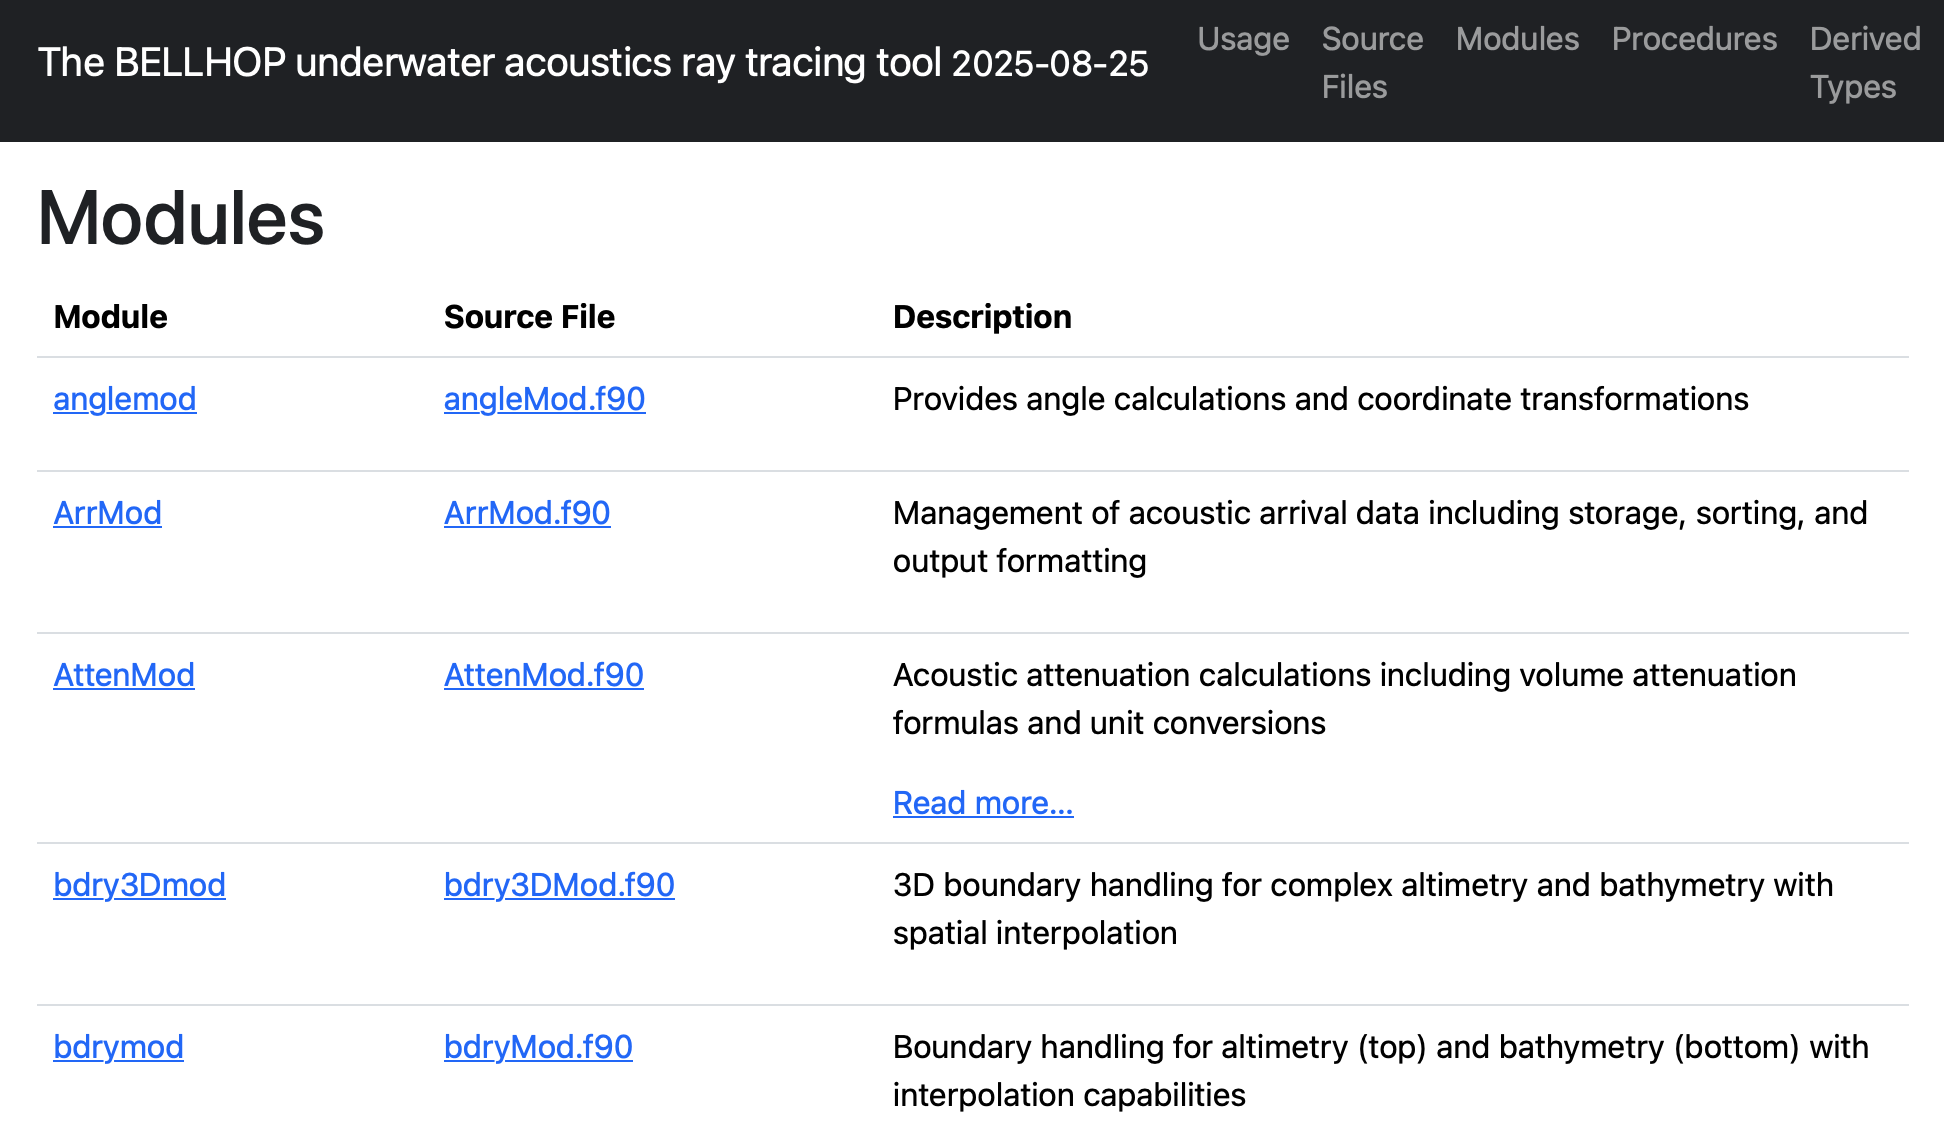
\includegraphics[width=0.45\linewidth]{fig/ford-modules-snap.png}\hfil
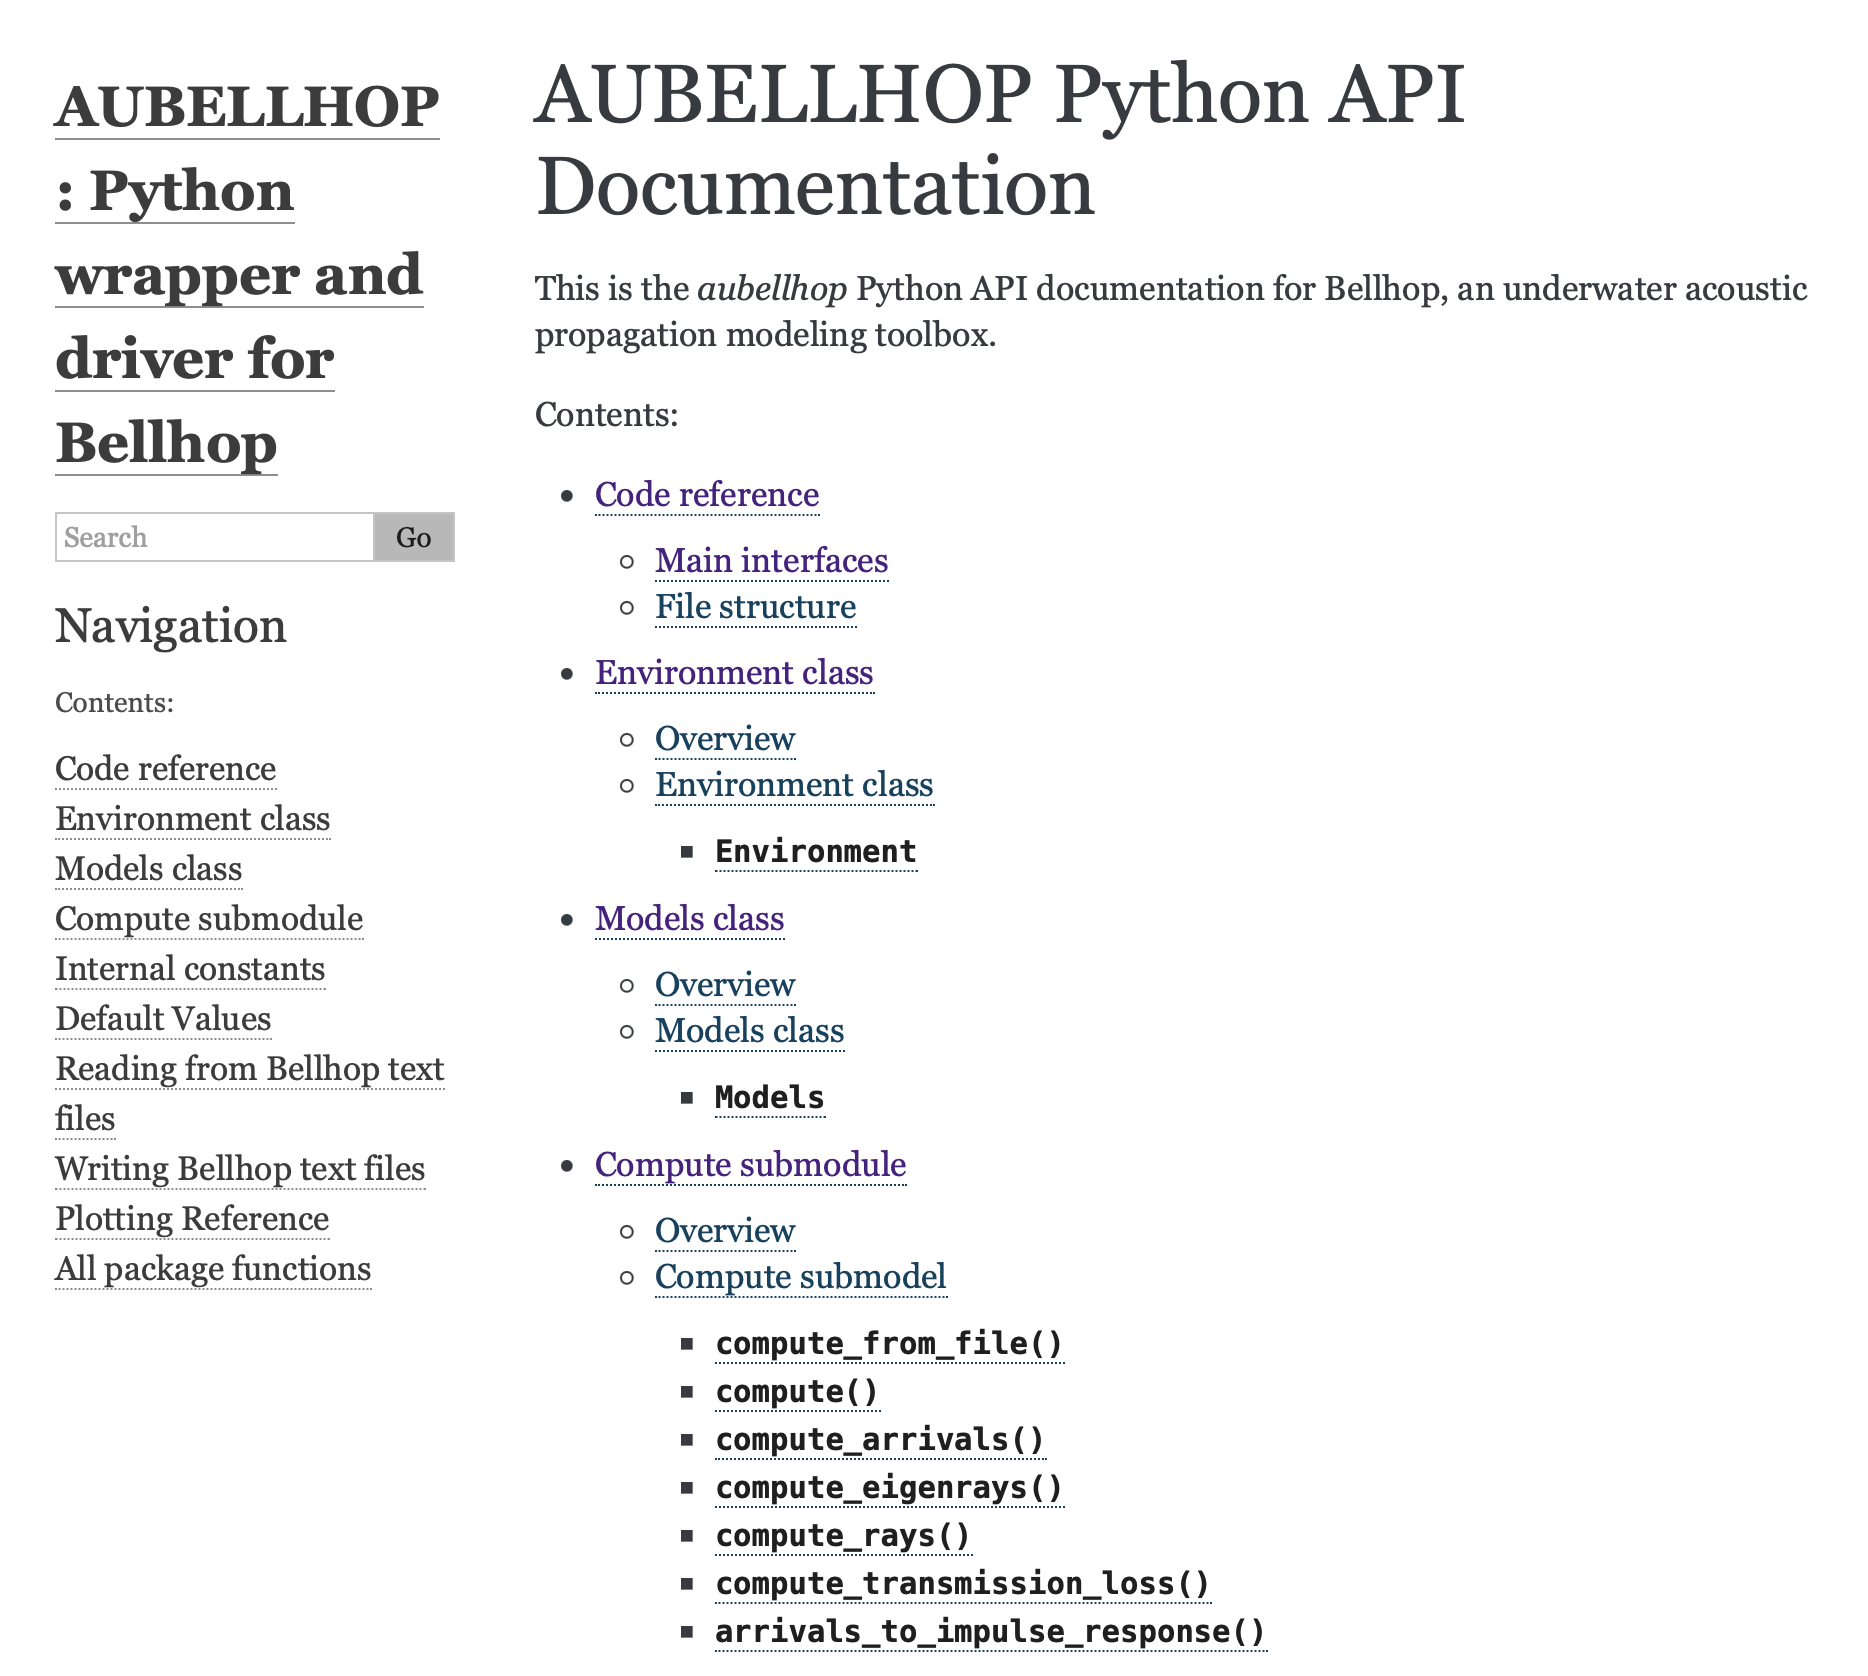
\includegraphics[width=0.45\linewidth]{fig/api}
\caption{Example output of the FORD Fortran Modules documentation (left) and the Sphinx Python API documentation (right).}
\end{figure}
\end{frame}

\begin{frame}
\frametitle{Online documentation}
\begin{figure}
\centerline{\fbox{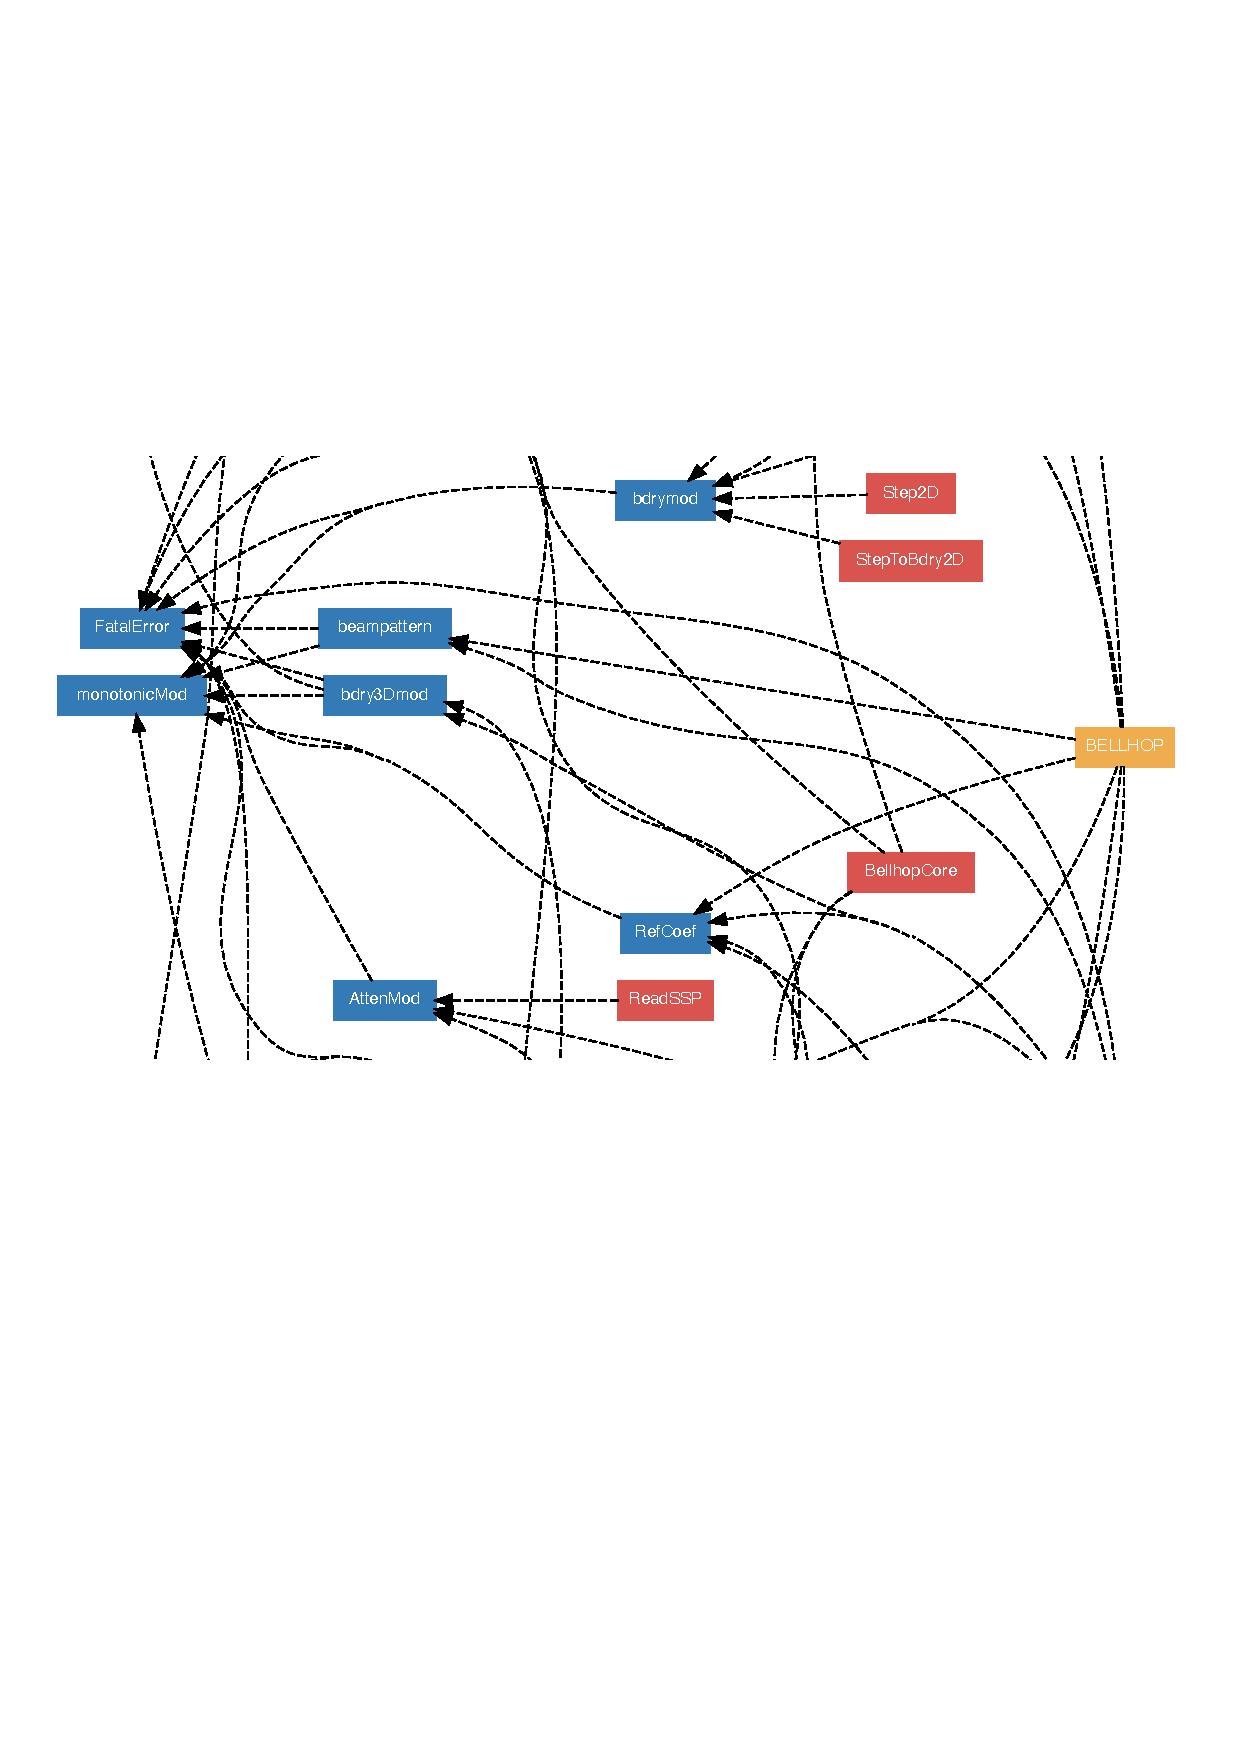
\includegraphics[width=0.8\linewidth]{fig/graphvis}}}
\caption{Extract from part of the automatically-generated Graphvis output from the FORD Modules documentation.}
\end{figure}
\end{frame}

\begin{frame}
\frametitle{Code coverage}
\begin{figure}
\centering
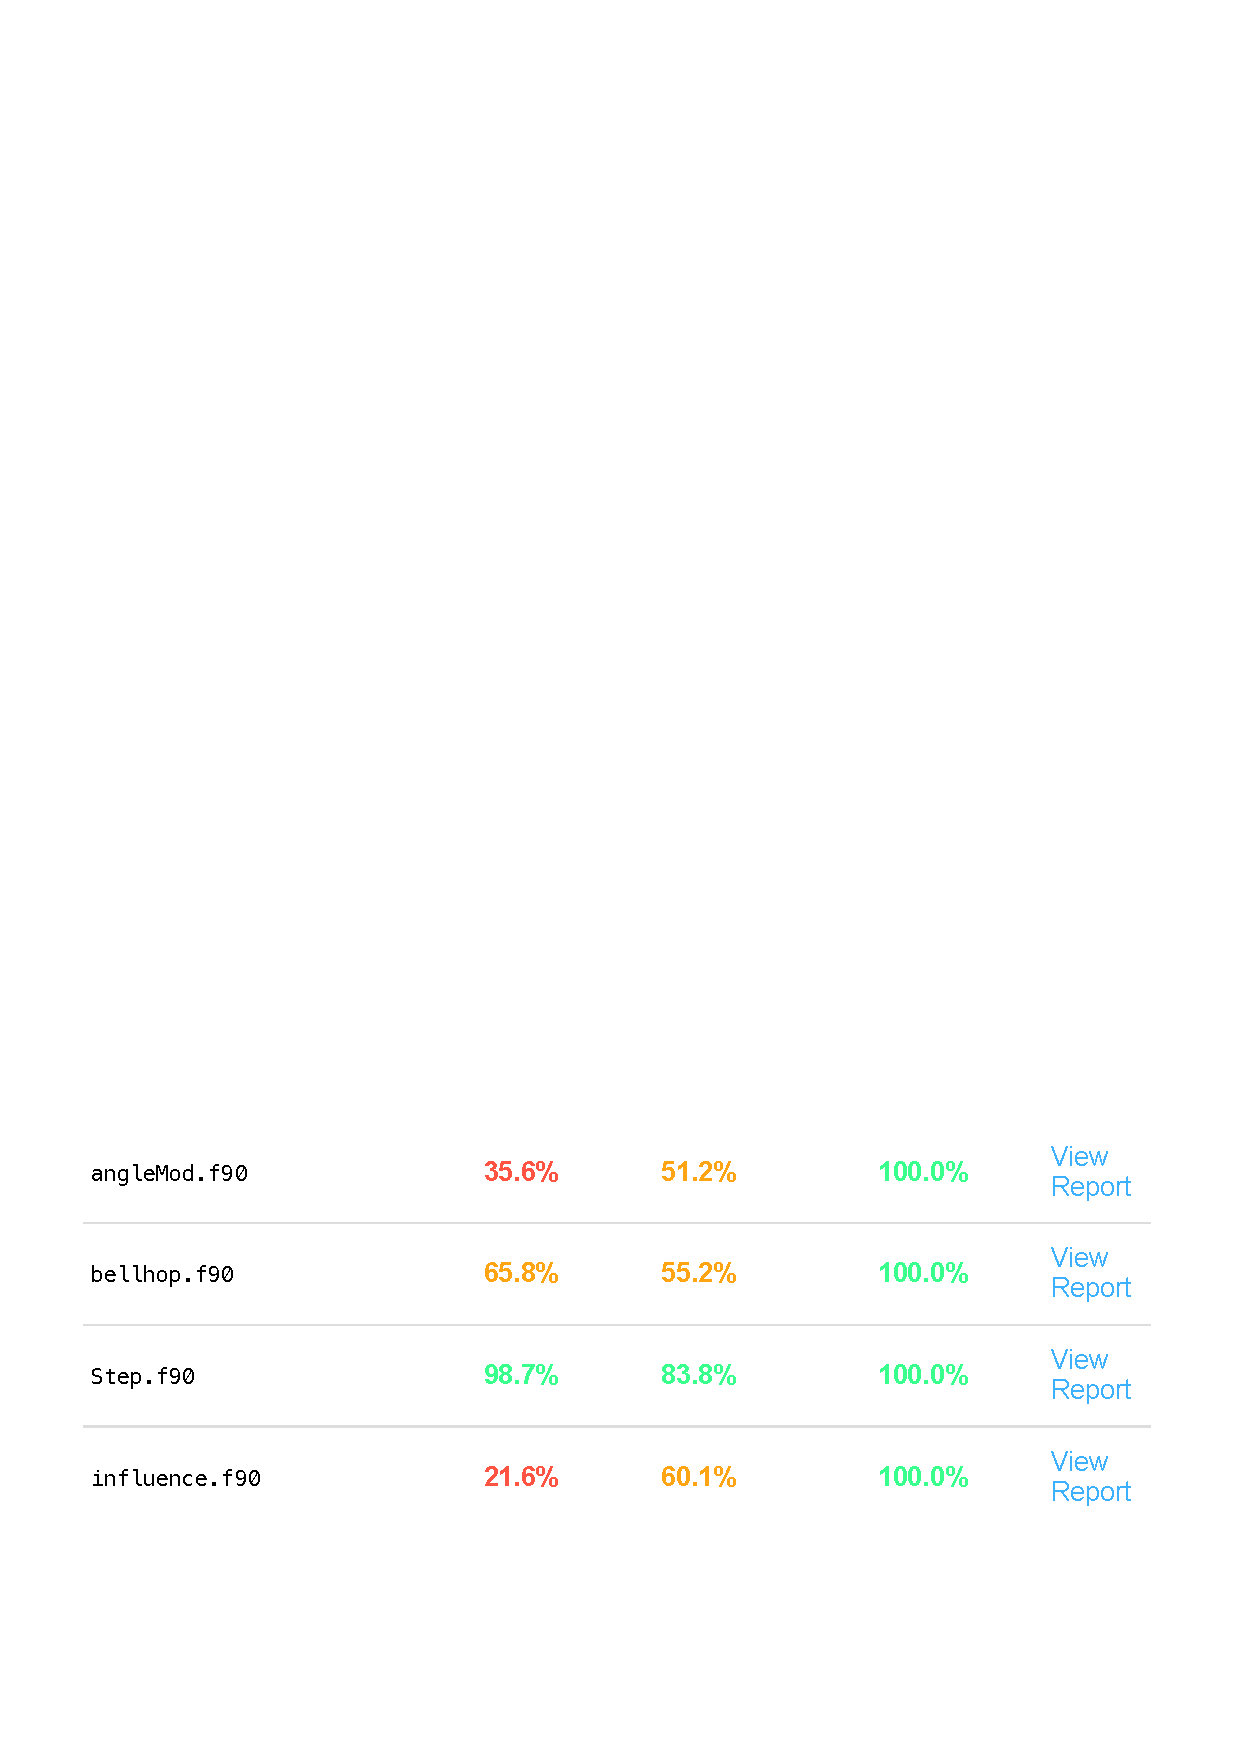
\includegraphics[width=0.8\linewidth]{fig/coverage.pdf}
\bigskip
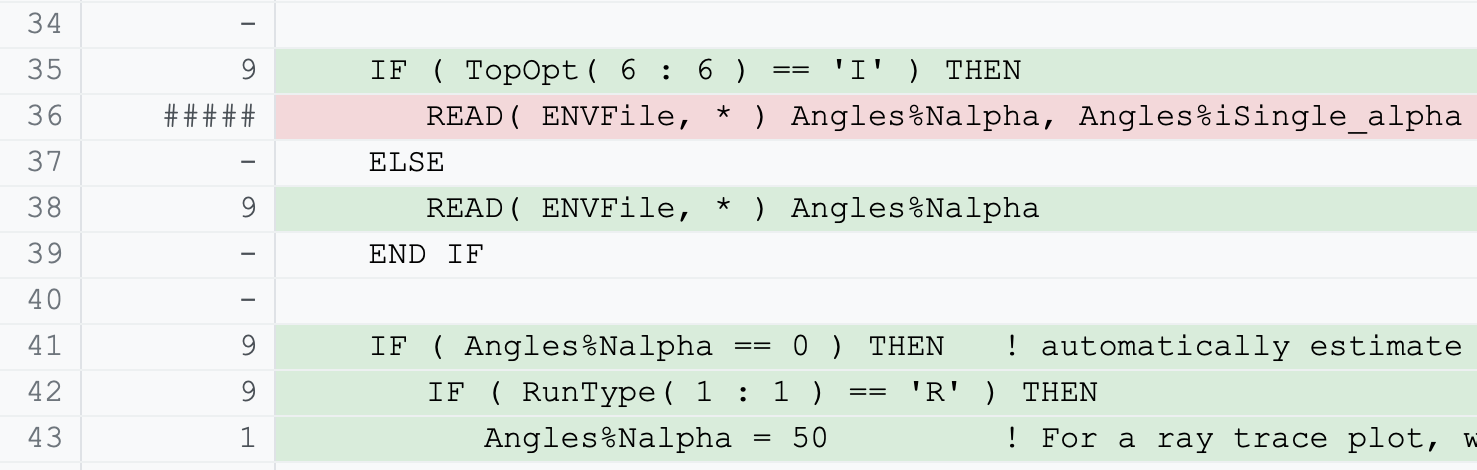
\includegraphics[width=0.8\linewidth]{fig/cov-detailed}
\caption{Example of coverage report summary output (top) and detailed per-file output (bottom).}
\end{figure}
\end{frame}

\begin{frame}
\frametitle{Tutorials}
\begin{figure}
\centering
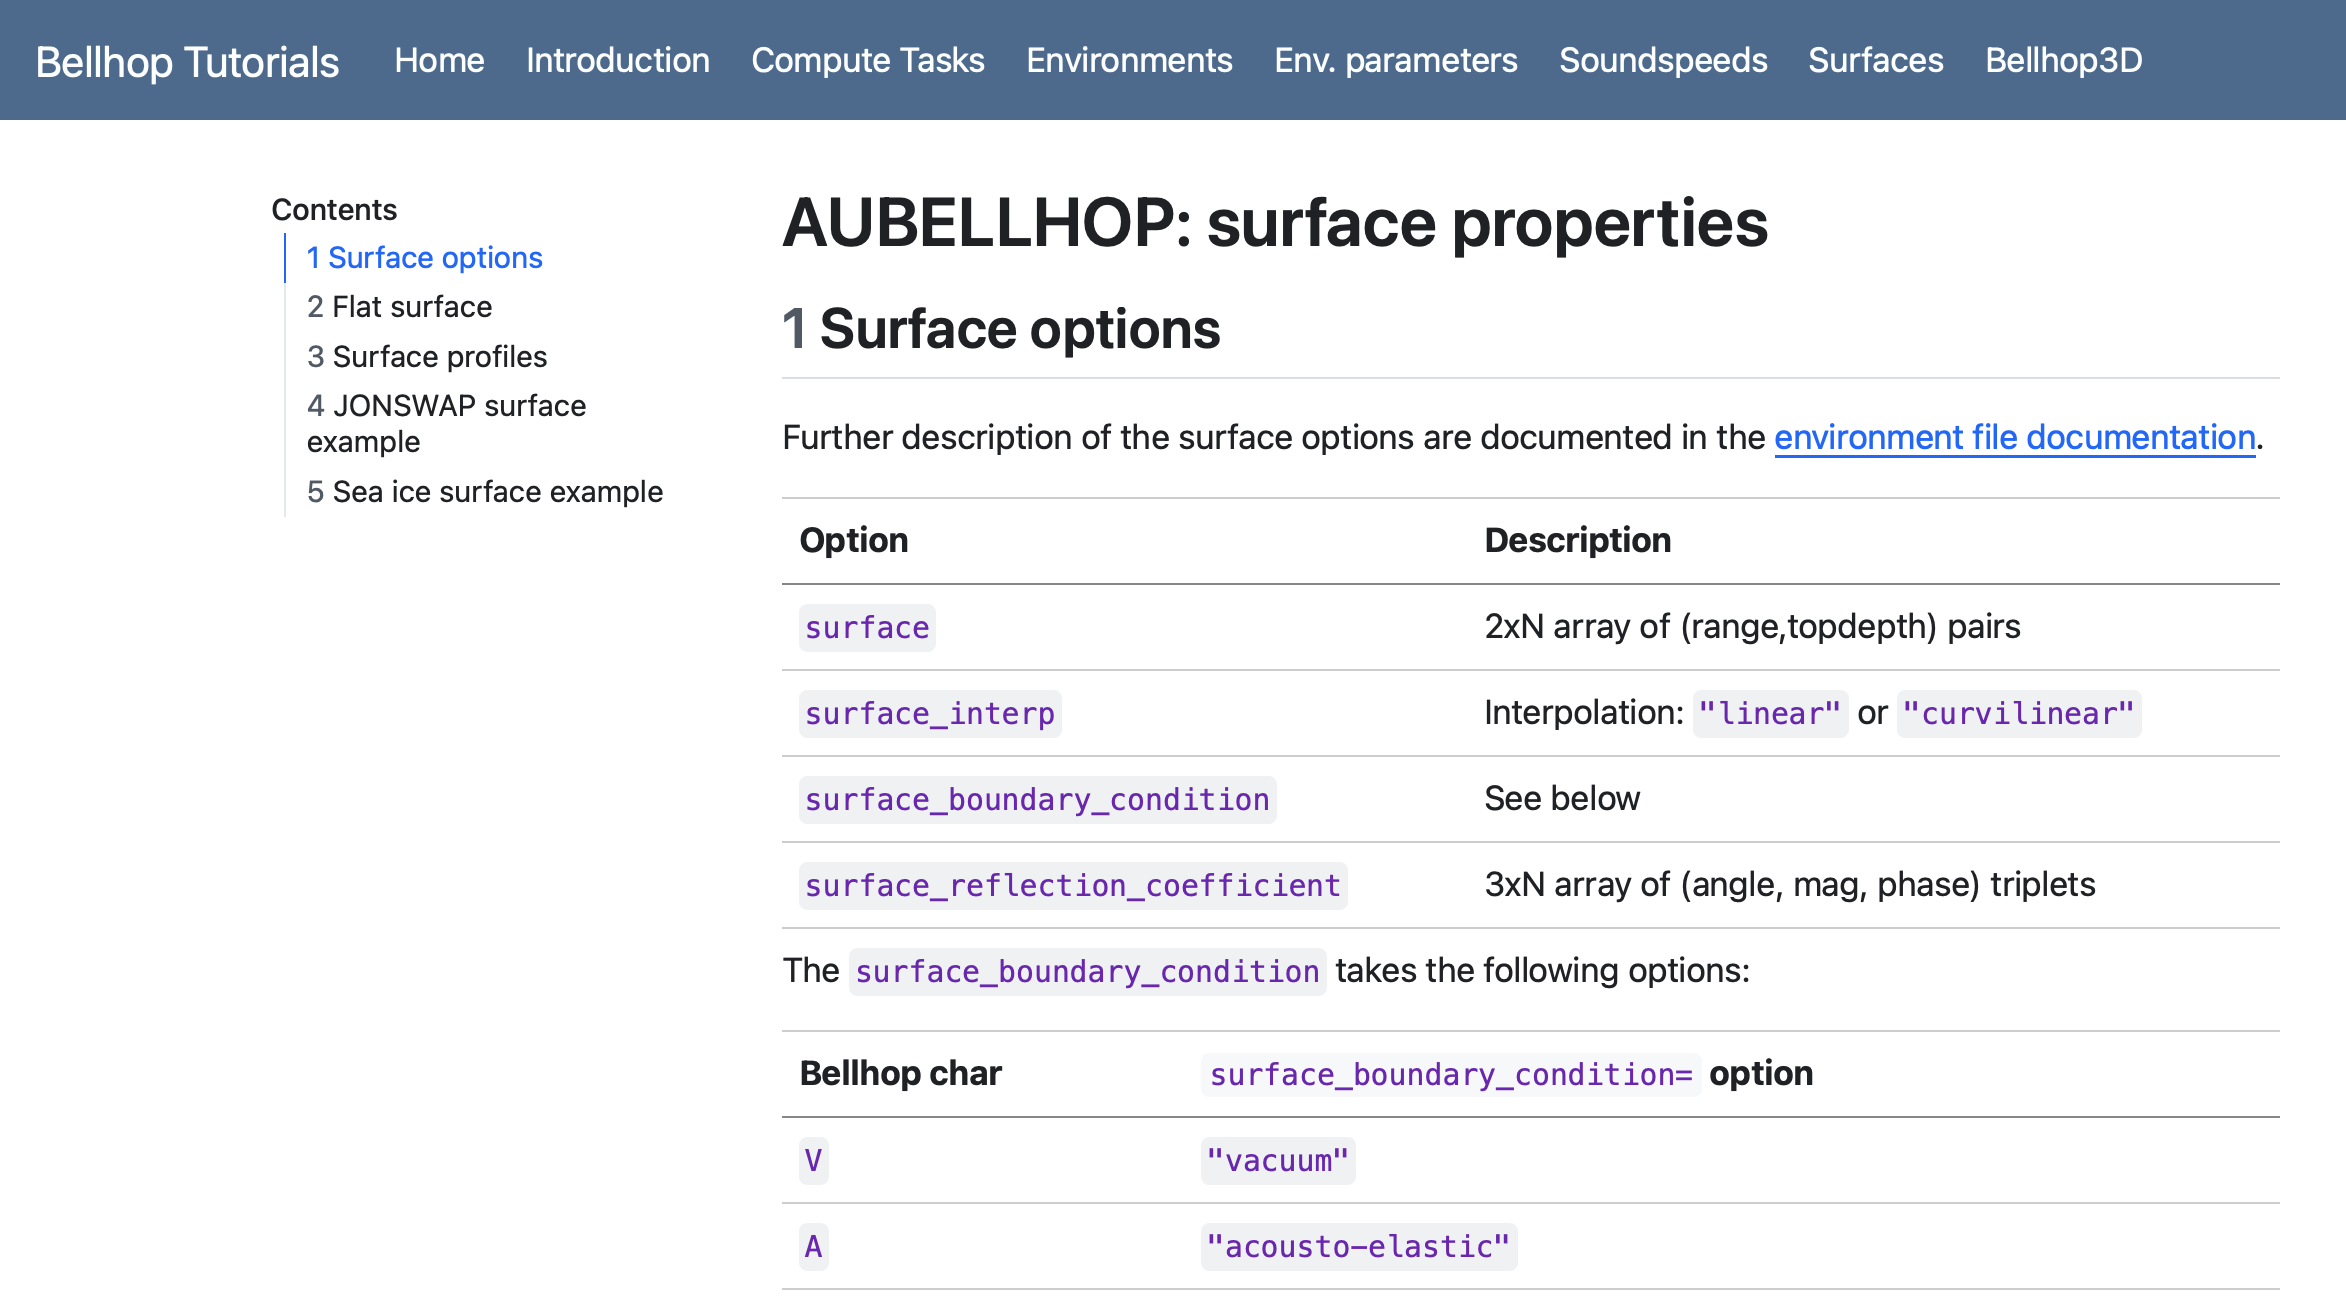
\includegraphics[width=0.8\linewidth]{fig/tute.png}
\caption{Example of `tutorial' documentation.}
\end{figure}

\end{frame}

\section{Outlook}

\begin{frame}
\sectionpage
\end{frame}

\begin{frame}
\frametitle{Further improvements}
\begin{itemize}
\item Build more explicit support for \texttt{bellhopcpp} and \texttt{bellhopcuda}
\item Provide direct wrapper for parallel execution
\begin{itemize}
\item Parallelise by engine, by environment, by depth, by ray, \dots
\end{itemize}
\item Complete test suite to 100\% coverage
\item Explore extensions to the Fortran code
\begin{itemize}
\item Bellhop2D and Bellhop3D do not quite have feature parity 
\item Changes should be made cautiously to avoid breaking compatibility
\end{itemize}
\end{itemize}
\end{frame}

\begin{frame}
\frametitle{Use of AI}
\begin{itemize}
\item Engineering software development is being democratised by AI
\item Need to carefully validate everything we do
\item AI was used in this project to help guide the Python development (best practices), debug tool chains, but all in supervised ways with extensive human input
\end{itemize}
\end{frame}

\begin{frame}
\frametitle{Conclusion}
\begin{itemize}
\item Ray/beam tracing is not the only underwater acoustics propagation method but it remains useful
\item What started as a hobby took on a life of its own
\item Hopefully others will find this useful too
\item If not, it's been a fun learning experience
\end{itemize}
\bigskip
A huge thank you to all the contributors to Bellhop over the decades
\end{frame}

\begin{frame}
\frametitle{References}
\begin{multicols}{3}
\printbibliography
\end{multicols}
\end{frame}

\end{document}


